\section{System Performance Analysis}
\label{sec:system_performance_analysis}

\newcommand{\TMAMotionSettings}{\href{https://rubinobs.atlassian.net/wiki/spaces/LSSTCOM/pages/53741249/TMA+Motion+Settings}{TMA Motion Settings}\xspace}
\newcommand{\testCase}[1]{\href{https://rubinobs.atlassian.net/projects/BLOCK?selectedItem=com.atlassian.plugins.atlassian-connect-plugin:com.kanoah.test-manager__main-project-page\#!/v2/testCase/#1}{#1}}

Topics to convert into text

\begin{itemize}
    \item M1M3 and M2 glass installed on the Simonyi Survey Telescope.
    \item Since then, we have been operating the telescope with limited velocity,
    acceleration, and jerk limits following the performances defined in \TMAMotionSettings.
    \item For each configuration, defined in terms of a percentage of the maximum
    velocity, acceleration, and jerk, we ran multiple gateway tests.
    \item The gateway tests are described in the \secRef{gateway_tests} below.
\end{itemize}

\subsection{Gateway Tests}
\label{sec:gateway_tests}

We started the ComCam on Sky test campaign using Simonyi Telescope with limited
performance, described as a percentage of the maximum velocity, acceleration,
and jerk limits. The performance is defined in \TMAMotionSettings Confluence page.

Before we can increase the telescope performance, we need to perform a set of
tests that ensure that the system will respond safely to the new velocity, acceleration,
and jerk. These tests are called gateway tests. Here is the list of all the tests.

\begin{itemize}
    \item \testCase{BLOCK-T227} Dynamic Tests at El = 34º short and long slews
    \item \testCase{BLOCK-T294} Dynamic Tests at El = 70º short and long slews
    \item \testCase{BLOCK-T231} TMA Azimuth Brake Test
    \item \testCase{BLOCK-T240} TMA Elevation Brake Distance
    \item \testCase{BLOCK-T241} M2 closed-loop break-out brake test during TMA slew
\end{itemize}


\subsubsection{Long and short slews at different elevations}
\label{subsubsec:long_and_short_slews}

These tests ensure that the force balance systems on M1M3 and on M2 can protect
the mirrors on different telescope positions and while slewing. As we increase
velocity, acceleration, and jerk limits, both mirrors suffer higher inertial
forces and the force actuators must counteract them.

%% TODO @b1quint - Ask Pablo, Holger, and Gabriele about the criteria for the
%% force balance systems for M2.
% For M1M3, the criteria is to keep the measured forces on the hardpoint actuators
% below the operational limit (15\% the breakaway limit). For M2, the criteria is
% ??????? (check with Holger, Gabriele, and Pablo).

The last set of data was collected on 2024-11-28. \figRef{block227_293_azel_slews}
shows the
slews performed when collecting this data starting at higher elevations (70$^\circ$)
and then moving to lower elevations (34$^\circ$).

\begin{center}
  \begin{figure}
    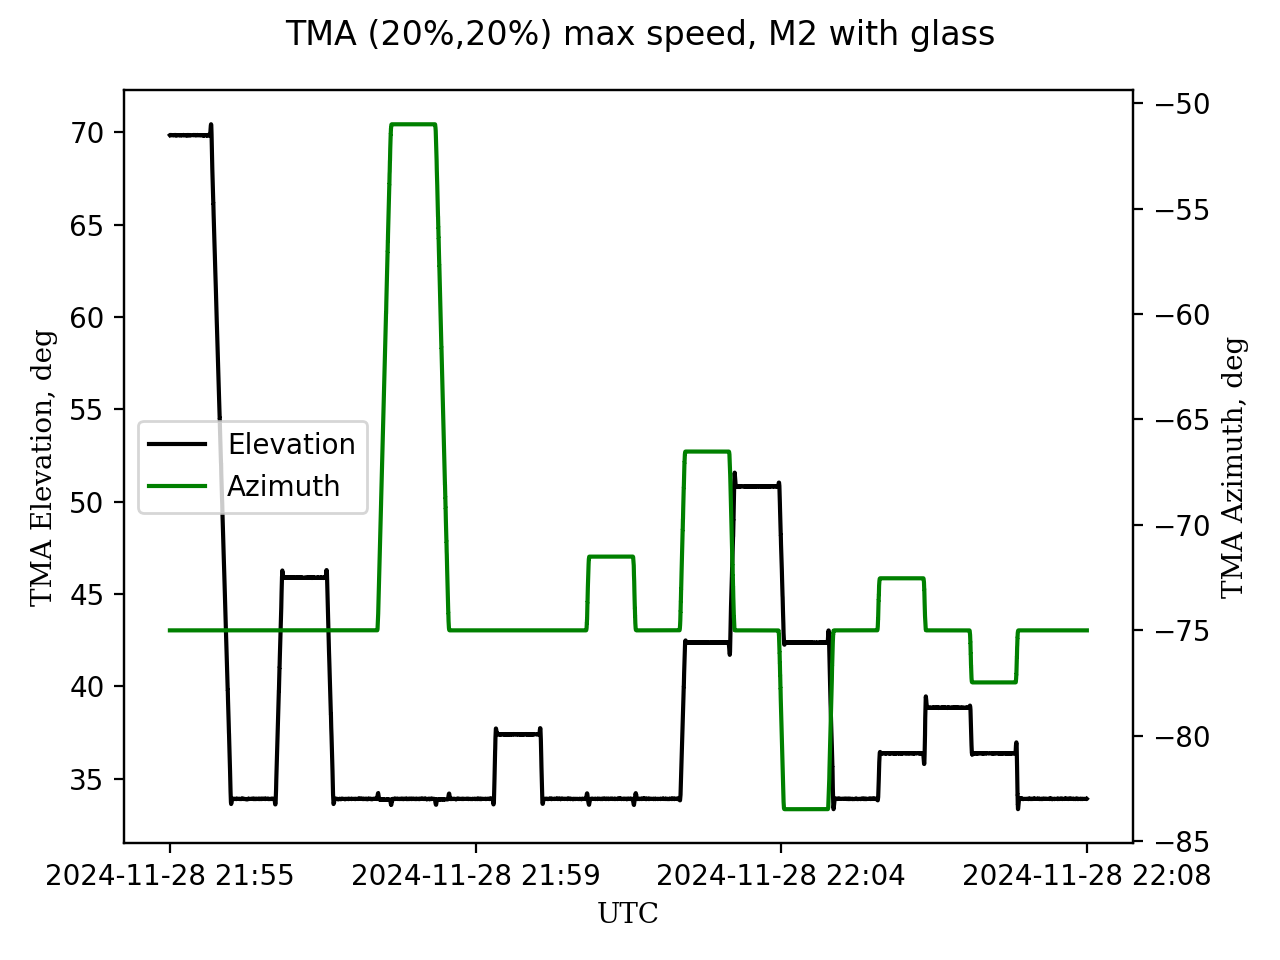
\includegraphics[width=0.5\textwidth]{spa/20_vel_acc_jerk/BLOCK-T227_azel_slews.png}
    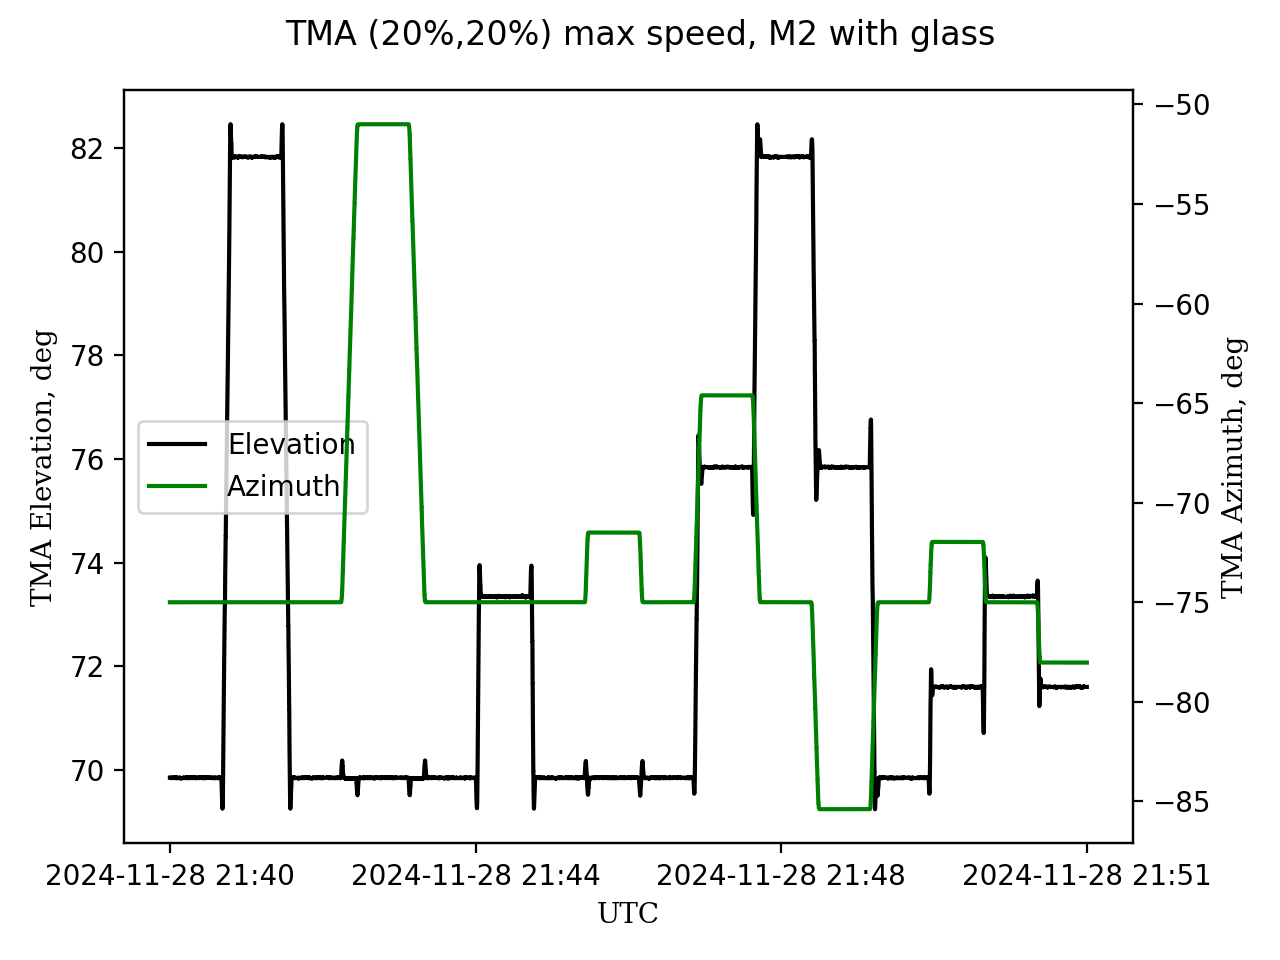
\includegraphics[width=0.5\textwidth]{spa/20_vel_acc_jerk/BLOCK-T293_azel_slews.png}
    \caption{TMA Short and Long slews at El = 34$^\circ$ (left) and El = 70$^\circ$ (right).}
    \label{fig:block227_293_azel_slews}
  \end{figure}
\end{center}

For each of these slews, the force balance system on M1M3 should keep the forces
measured on the hardpoints below an operational limit (15\% of the breakaway limit, nominally 450 N).
\figRefII{block227_m1m3_hp_histograms}{block293_m1m3_hp_histograms}
show histograms with the number of slews that hit certain minima
and maxima values for the hardpoint forces. The left histogram shows the minima
reached on each slew. The right histogram shows the maxima reached on each slew.
The red dashed lines show the fatigue limit (30\% of the breakaway limit, nominally 900 N).

You can see a few slews with min/max reaching 800 N at low elevations.
This is quite close to fatigue limits (900 N).
However, these slews were performed without booster valves enabled.
In addition, the big majority of the slews have measured forces below the operational limit.
This gave us confidence that, from M1M3's perpective, we can use the 20\% velocity, acceleration, and jerk for the rest of the campaign.
Note that we ran a few test slews with booster valves enabled and loads were significantly reduced (<200N per HP) before we got faults in some of the actuators with bad valves (need data analysis).

\begin{figure}
    \centering
    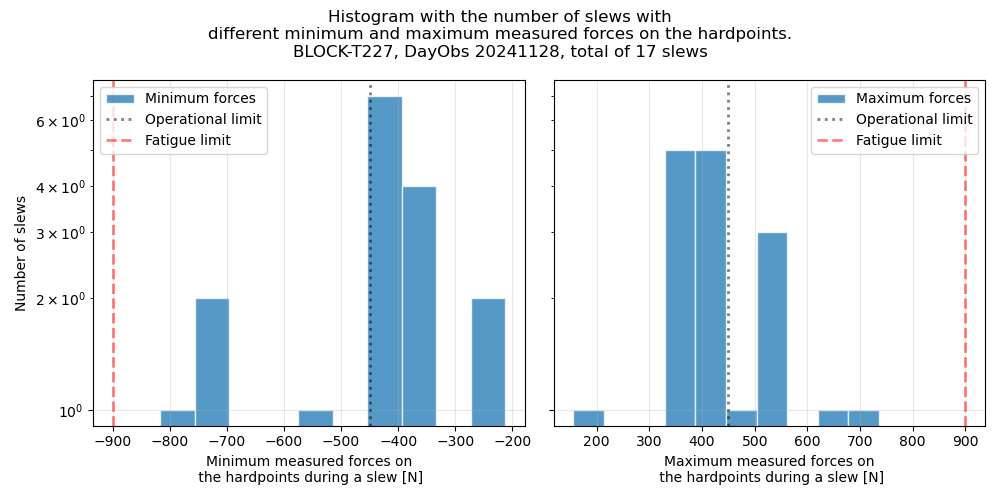
\includegraphics[width=0.8\textwidth]{spa/20_vel_acc_jerk/BLOCK-T227_m1m3_hp_histograms.png}
    \caption{M1M3 hardpoint histograms min/max HP forces at low elevation.}
    \label{fig:block227_m1m3_hp_histograms}
    \end{figure}

\begin{figure}
    \centering
    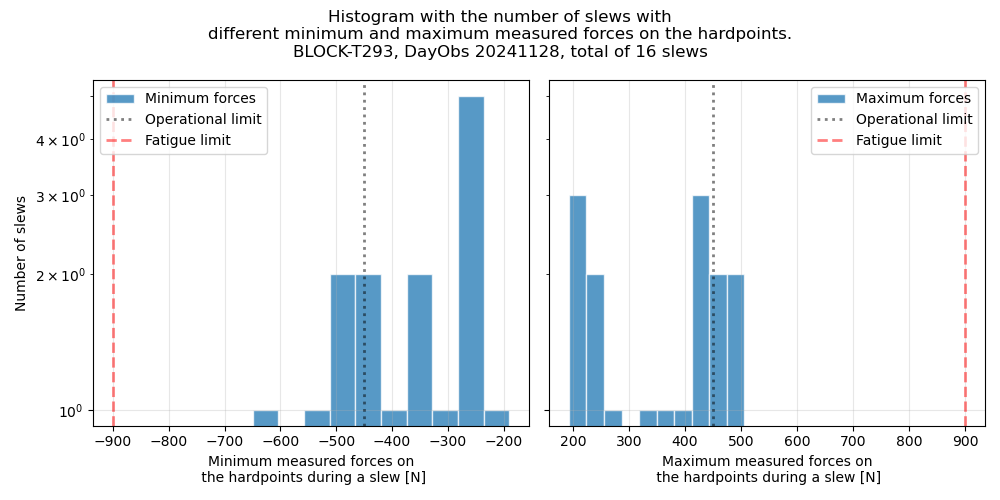
\includegraphics[width=0.8\textwidth]{spa/20_vel_acc_jerk/BLOCK-T293_m1m3_hp_histograms.png}
    \caption{M1M3 hardpoint histograms min/max HP forces at high elevation.}
    \label{fig:block293_m1m3_hp_histograms}
    \end{figure}

Similarly, M2 has limits of the measured forces associated with its closed loop and its
open loop.
\figRefIII{m2_axial_measured_forces}{m2_tangent_measured_forces}{m2_tangent_force_errors}
show the axial forces, the tangent forces, and the tangent
force errors for the slews performed at different elevations. We can see that, for every slew,
all the forces are within the closed loop maximum forces limit. This means that, from M2's
perpective, we are safe to operate the telescope with 20\% velocity, acceleration, and jerk.

\begin{figure}
    \centering
    \begin{subfigure}[b]{0.45\textwidth}
        \centering
        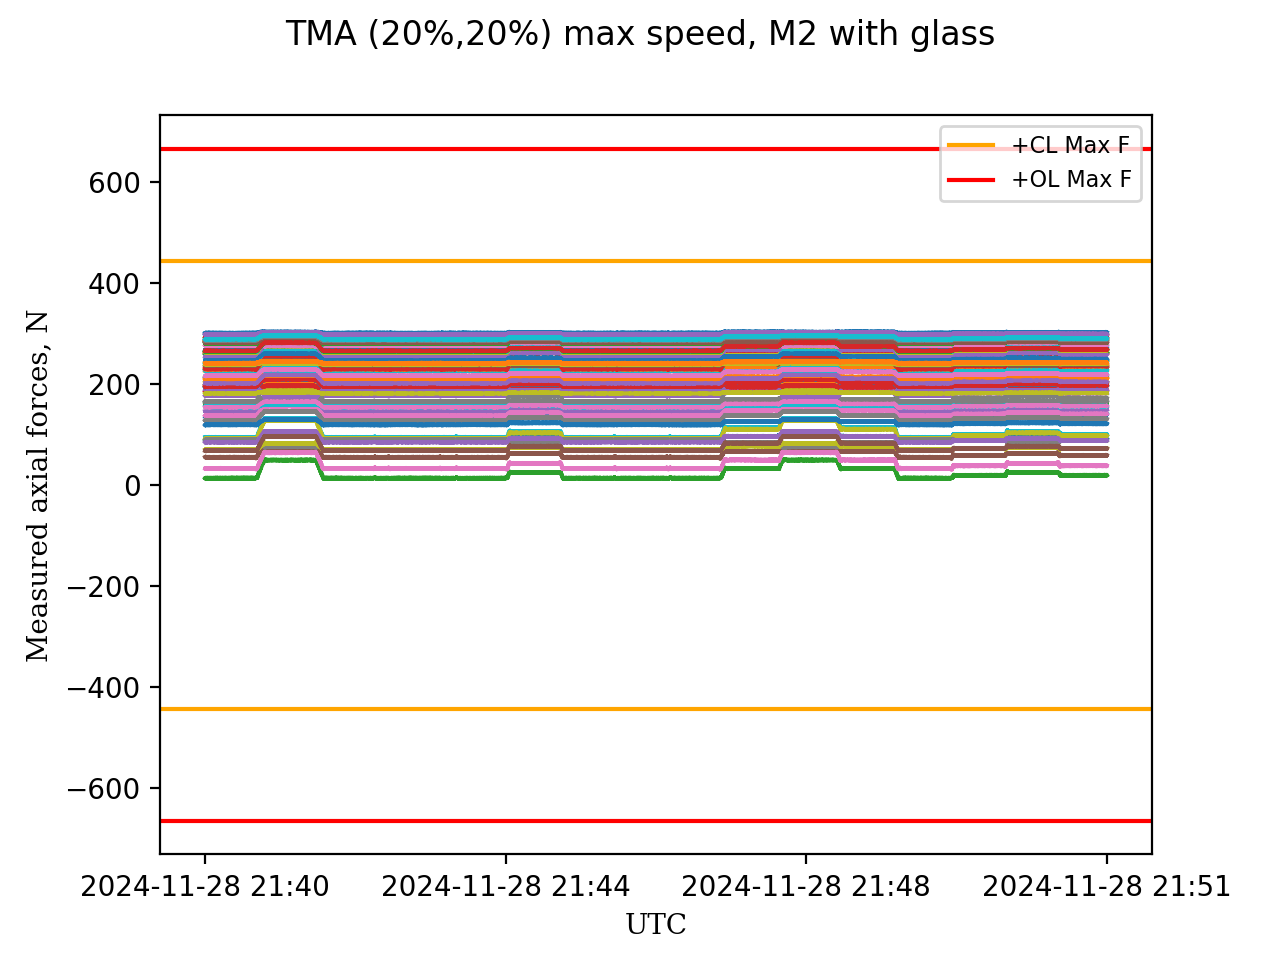
\includegraphics[width=\textwidth]{spa/20_vel_acc_jerk/BLOCK-T227_m2_axial_measured_forces.png}
        \caption{M2 axial measured forces at low elevation.}
        \label{fig:block227_m2_axial_measured_forces}
    \end{subfigure}
    \hfill
    \begin{subfigure}[b]{0.45\textwidth}
        \centering
        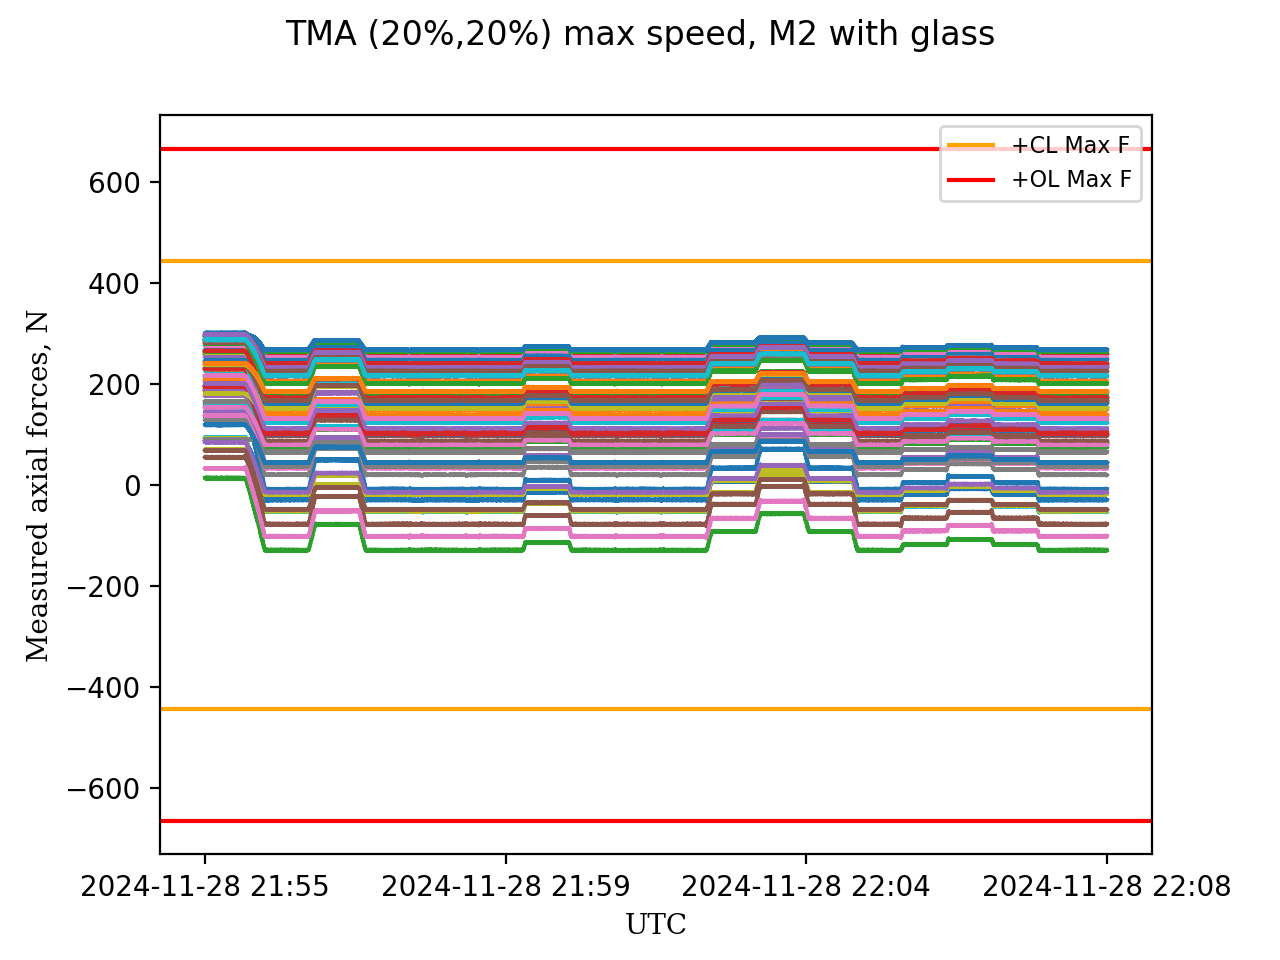
\includegraphics[width=\textwidth]{spa/20_vel_acc_jerk/BLOCK-T293_m2_axial_measured_forces.png}
        \caption{M2 axial measured forces at high elevation.}
        \label{fig:block293_m2_axial_measured_forces}
    \end{subfigure}
    \caption{M2 axial measured forces during the slews at different elevations.}
    \label{fig:m2_axial_measured_forces}
\end{figure}

\begin{figure}
    \centering
    \begin{subfigure}[b]{0.45\textwidth}
        \centering
        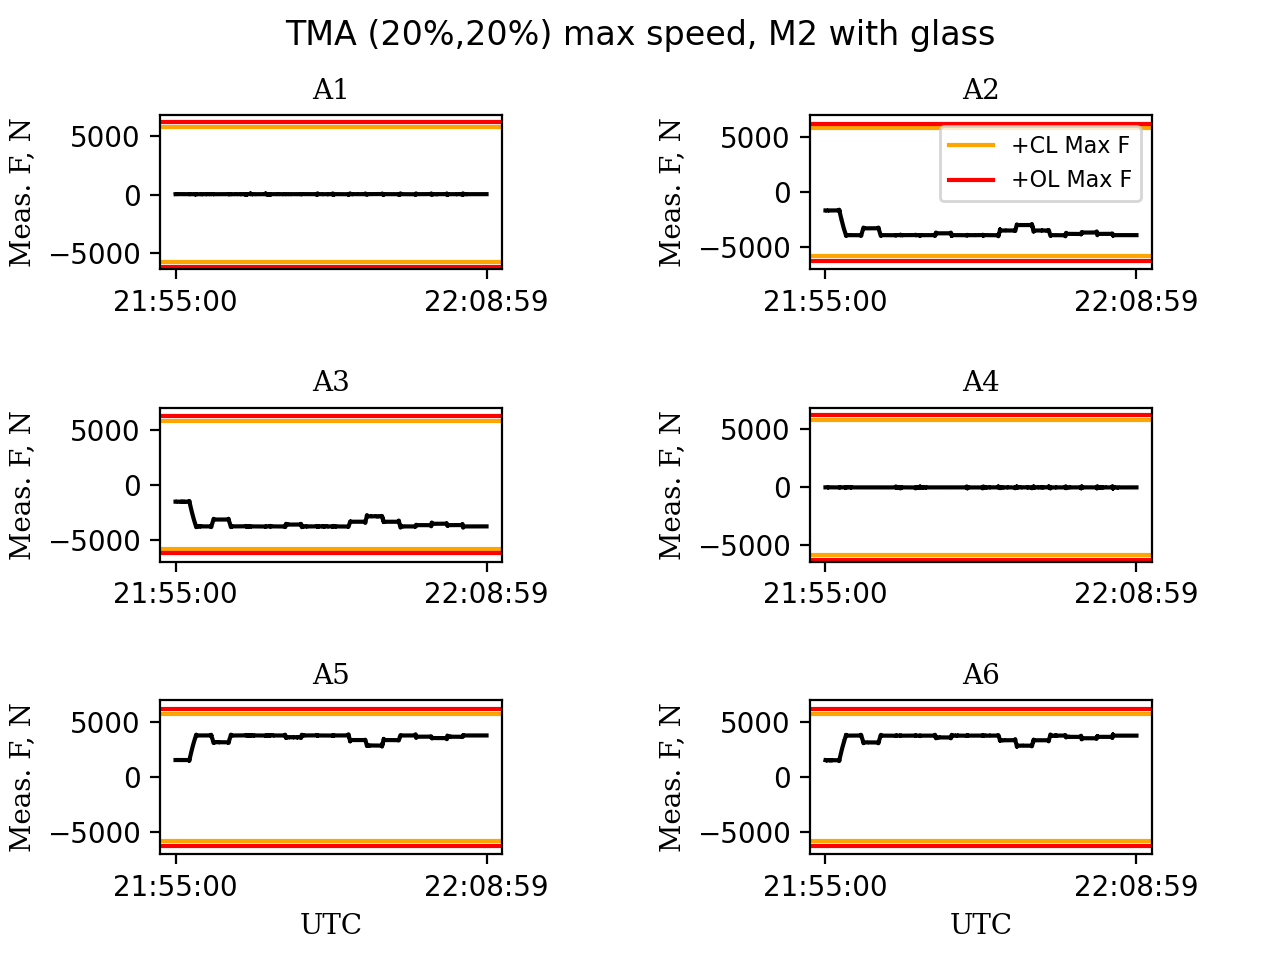
\includegraphics[width=\textwidth]{spa/20_vel_acc_jerk/BLOCK-T227_m2_tangent_measured_forces.png}
        \caption{M2 tangent force errors at low elevation.}
        \label{fig:block227_m2_tangent_measured_forces}
    \end{subfigure}
    \hfill
    \begin{subfigure}[b]{0.45\textwidth}
        \centering
        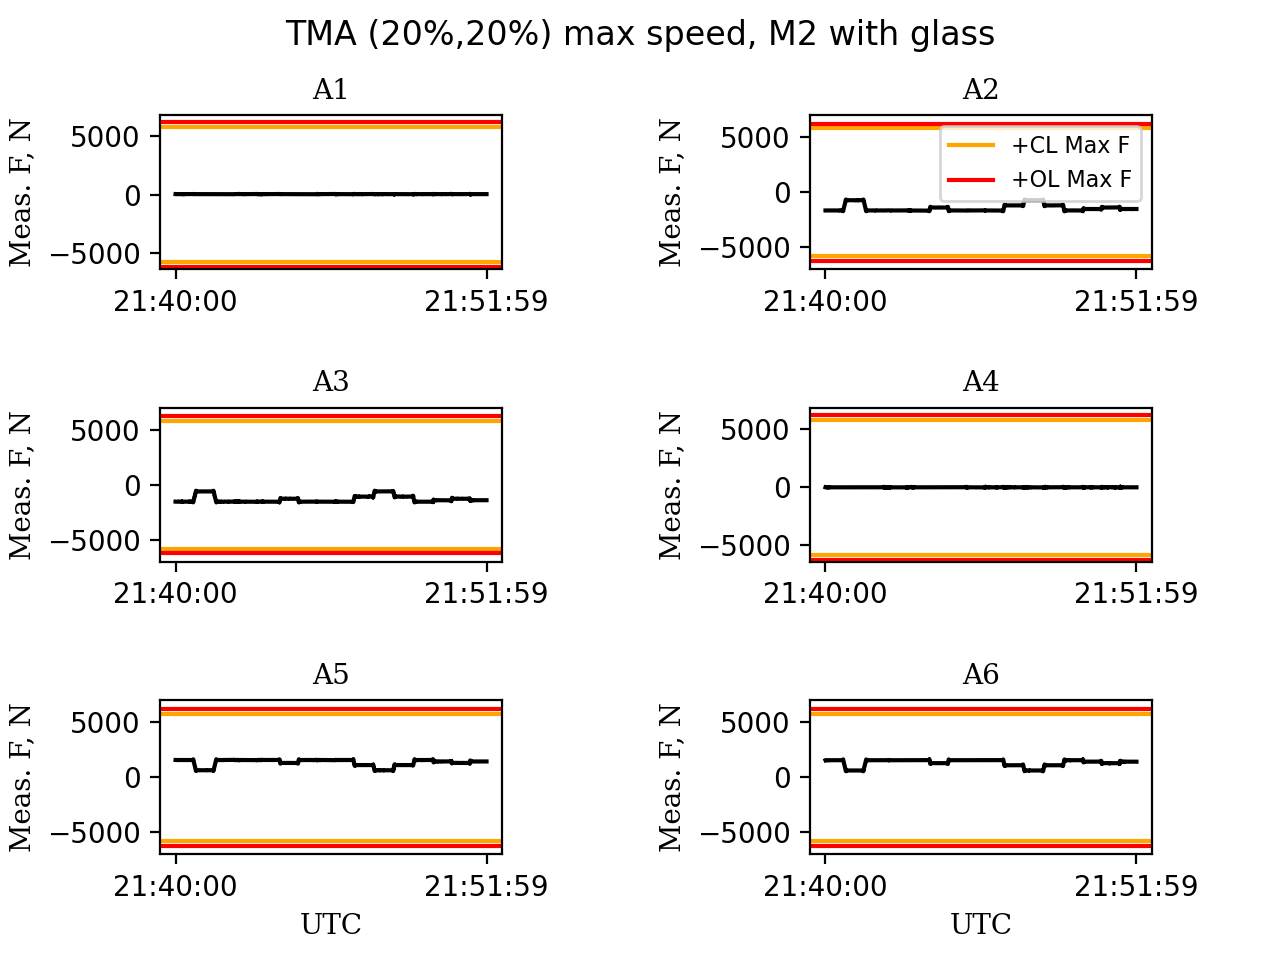
\includegraphics[width=\textwidth]{spa/20_vel_acc_jerk/BLOCK-T293_m2_tangent_measured_forces.png}
        \caption{M2 tangent force errors at high elevation.}
        \label{fig:block293_m2_tangent_measured_forces}
    \end{subfigure}
    \caption{M2 measured tangent forces during the slews at different elevations.}
    \label{fig:m2_tangent_measured_forces}
\end{figure}

\begin{figure}
    \centering
    \begin{subfigure}[b]{0.45\textwidth}
        \centering
        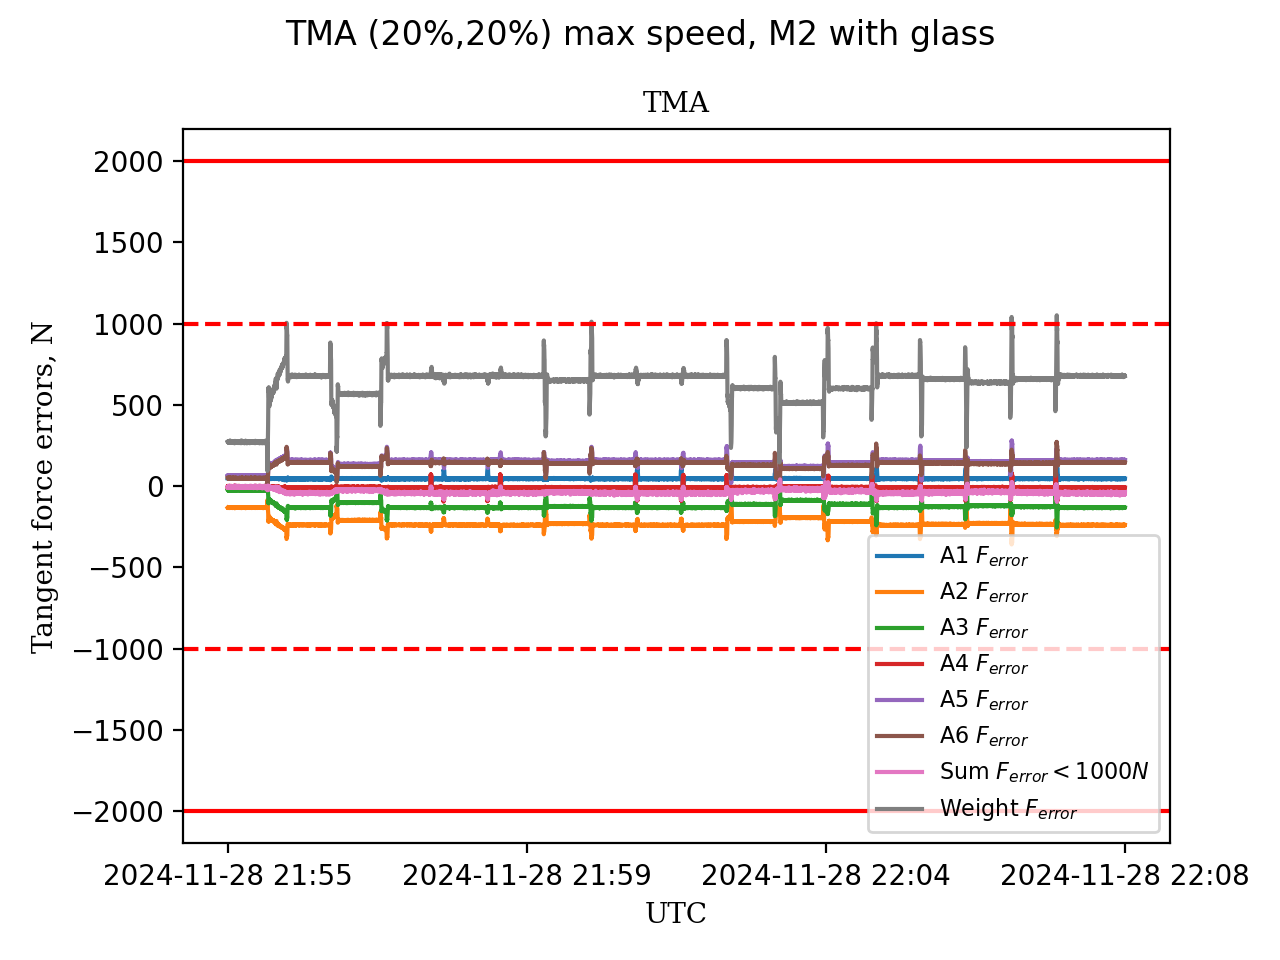
\includegraphics[width=\textwidth]{spa/20_vel_acc_jerk/BLOCK-T227_m2_tangent_force_errors.png}
        \caption{M2 tangent force errors at low elevation.}
        \label{fig:block227_m2_tangent_force_errors}
    \end{subfigure}
    \hfill
    \begin{subfigure}[b]{0.45\textwidth}
        \centering
        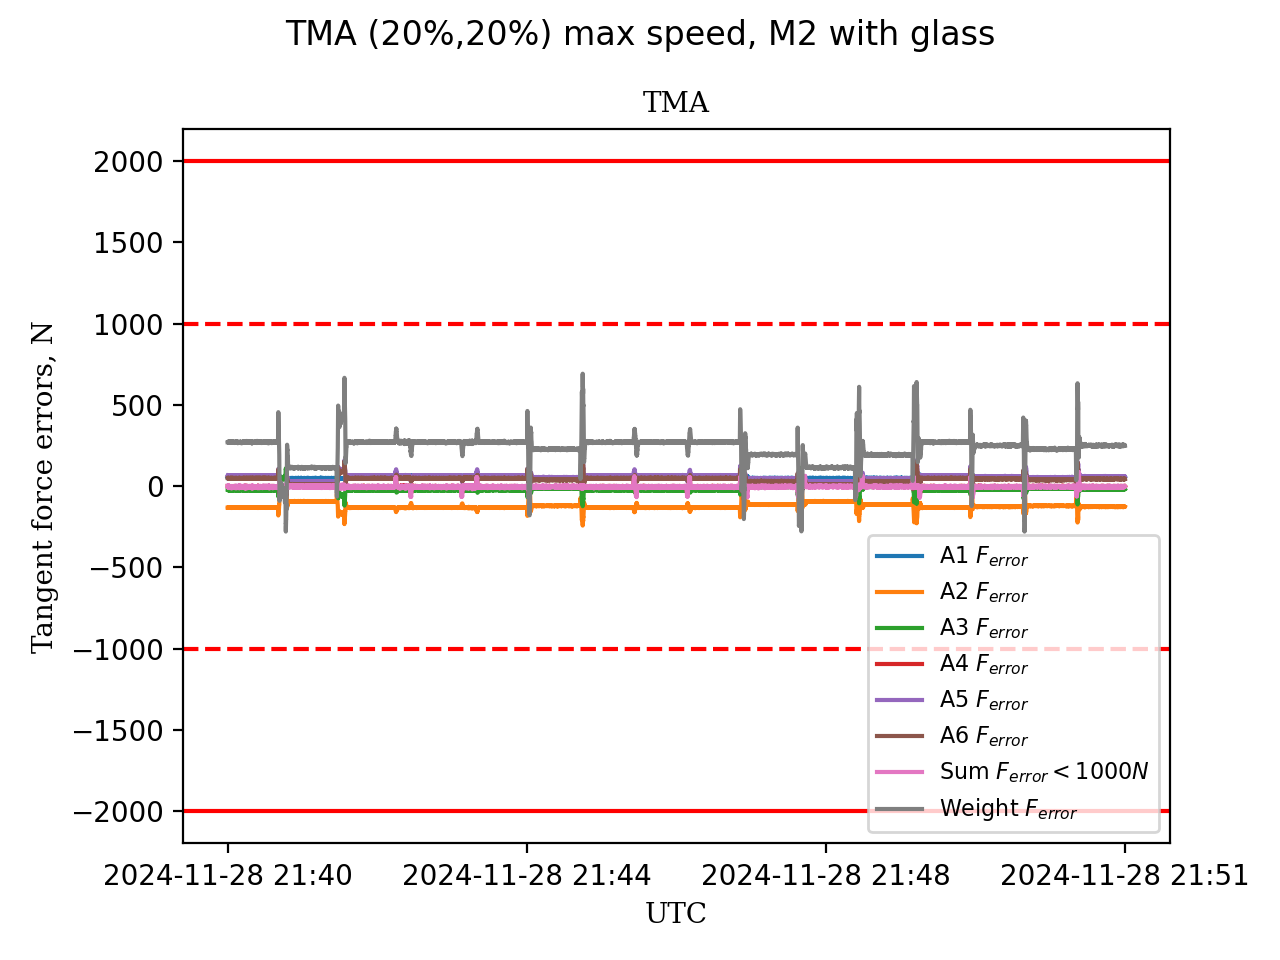
\includegraphics[width=\textwidth]{spa/20_vel_acc_jerk/BLOCK-T293_m2_tangent_force_errors.png}
        \caption{M2 tangent force errors at high elevation.}
        \label{fig:block293_m2_tangent_force_errors}
    \end{subfigure}
    \caption{M2 tangent force errors during the slews at different elevations.}
    \label{fig:m2_tangent_force_errors}
\end{figure}


\subsubsection{M2 close-loop breakout tests}
\label{subsubsec:m2_close_loop_breakout_tests}

\testCase{BLOCK-T241} M2 closed-loop break-out brake test during TMA slew is a test that
ensures that M2 can survive an event where the telescope is slewing and, for whatever reason,
the closed-loop system is disabled. In this case, the telescope will go to a fault and stop.

\figRefIII{block241_m2_axial_measured_forces}{block241_m2_tangent_measured_forces}{block241_m2_tangent_force_errors}
show the axial forces, the tangential forces, and the tangential force errors
during an event where the closed-loop system is disabled. The plots show that both axial and
tangential forces are within the limits. Considering this tests, we can say that M2 is safe to
operate with 20\% velocity, acceleration, and jerk.

\begin{figure}
    \centering
    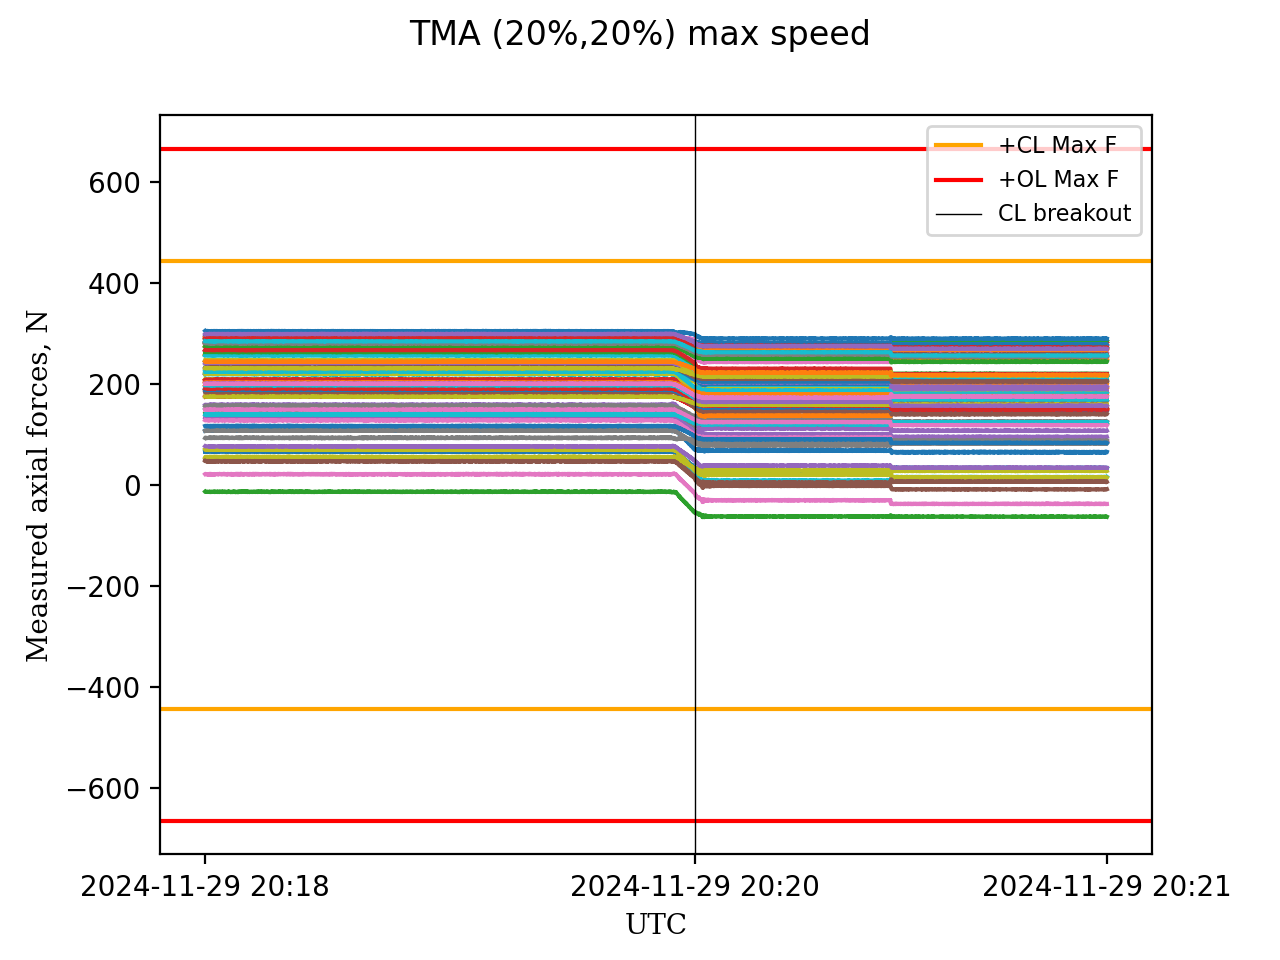
\includegraphics[width=0.8\textwidth]{spa/20_vel_acc_jerk/BLOCK-T241_m2_axial_measured_forces.png}
    \caption{M2 axial measured forces during the closed-loop break-out test.}
    \label{fig:block241_m2_axial_measured_forces}
    \end{figure}

\begin{figure}
    \centering
    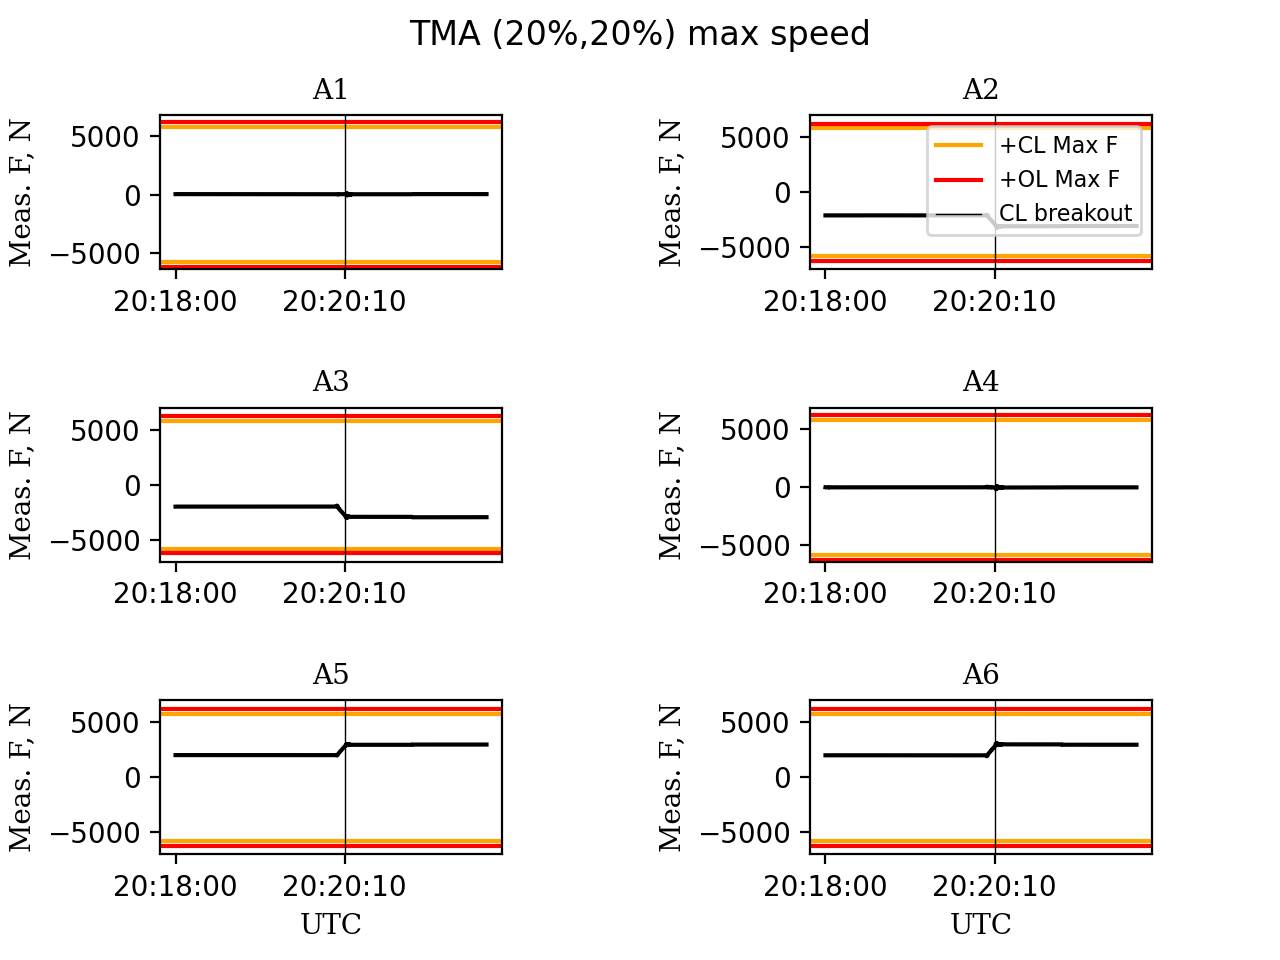
\includegraphics[width=0.8\textwidth]{spa/20_vel_acc_jerk/BLOCK-T241_m2_tangent_measured_forces.png}
    \caption{M2 tangential measured forces during the closed-loop break-out test.}
    \label{fig:block241_m2_tangent_measured_forces}
    \end{figure}

\begin{figure}
    \centering
    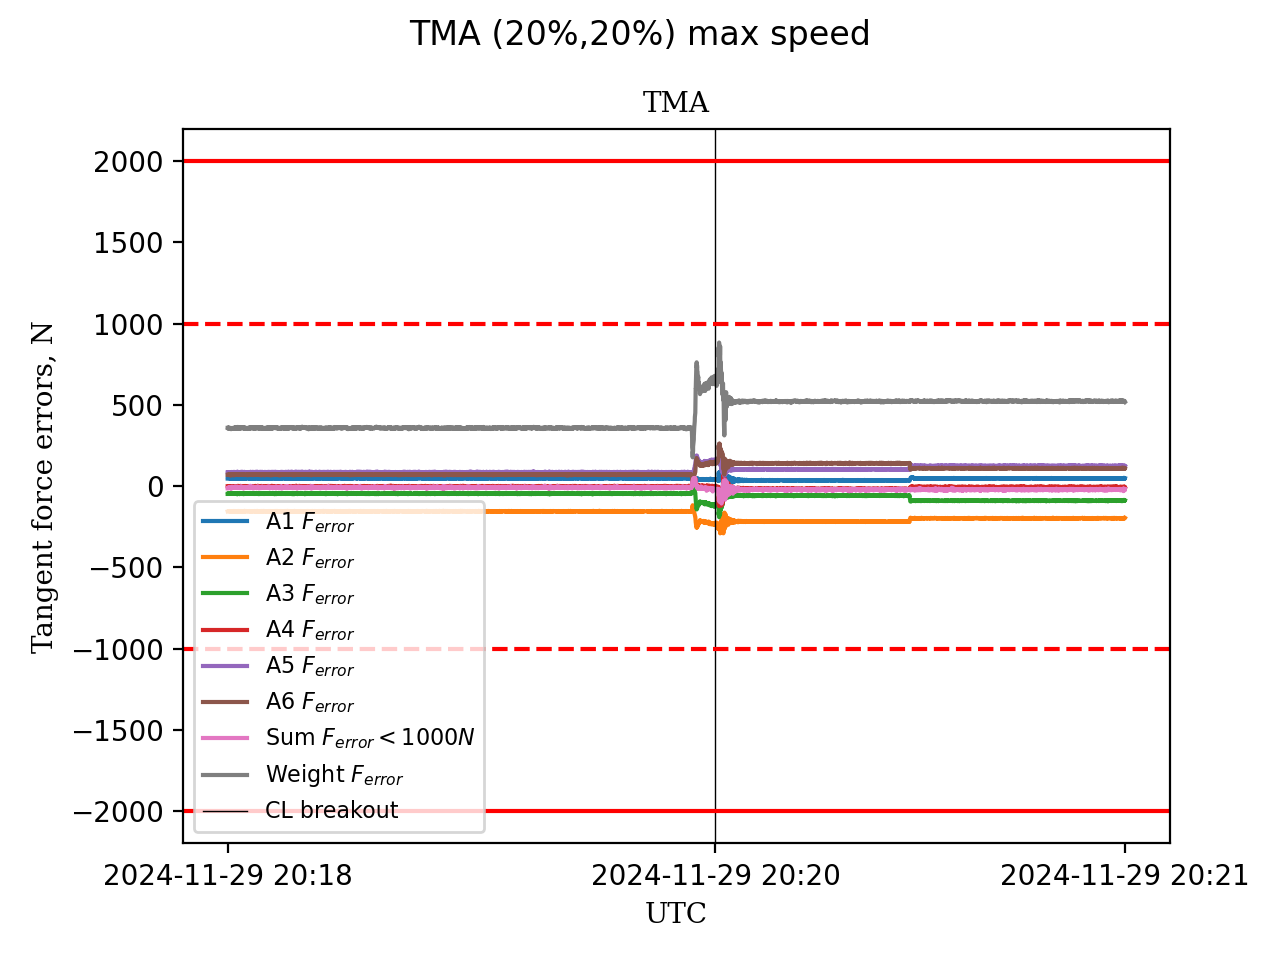
\includegraphics[width=0.8\textwidth]{spa/20_vel_acc_jerk/BLOCK-T241_m2_tangent_force_errors.png}
    \caption{M2 tangential force errors during the closed-loop break-out test.}
    \label{fig:block241_m2_tangent_force_errors}
    \end{figure}


\subsubsection{TMA azimuth and elevation brake tests}
\label{subsubsec:tma_azimuth_and_elevation_brake_tests}

The tests \testCase{BLOCK-T231} TMA Azimuth Brake Test and
\testCase{BLOCK-T240} TMA Elevation Brake Distance are designed to ensure that the
telescope will stop in case of an emergency. Accordingly to \figRef{block240_azEl_brake_distance}
the telescope travels 1.6 degrees in El (2.2 deg/s$^2$ peak deceleration) after the hard stop initiated.
In Az, it travels 1.9 degrees (3.9 deg/s$^2$ peak deceleration) after hard stop initiated.
Both without any mirror faults. These values seem reasonably low and confirm that the telescope
would be safe in case of an emergency.

\begin{figure}
  \centering
  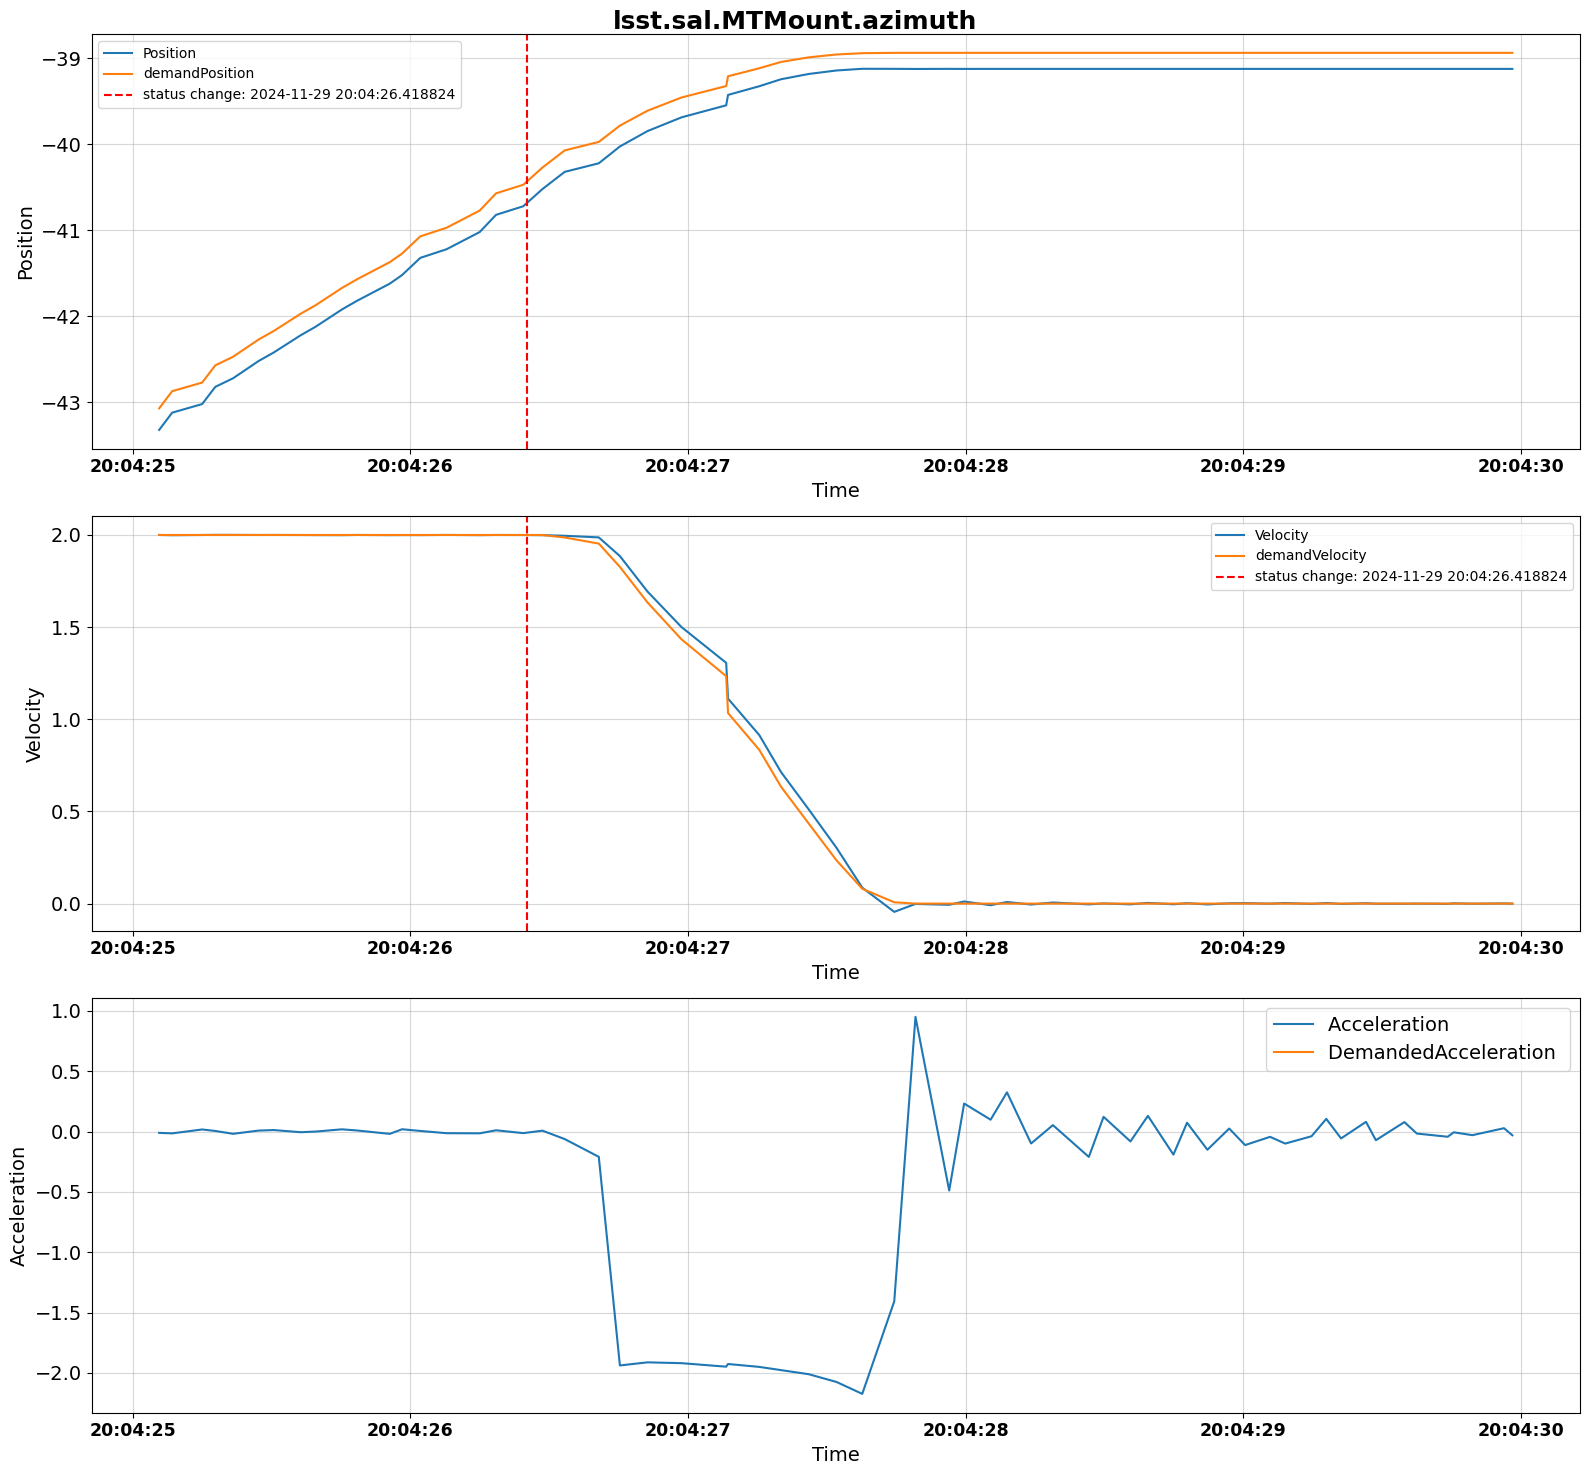
\includegraphics[width=0.45\textwidth]{spa/20_vel_acc_jerk/BLOCK-T231_az_brake_tests.png}
  \qquad
  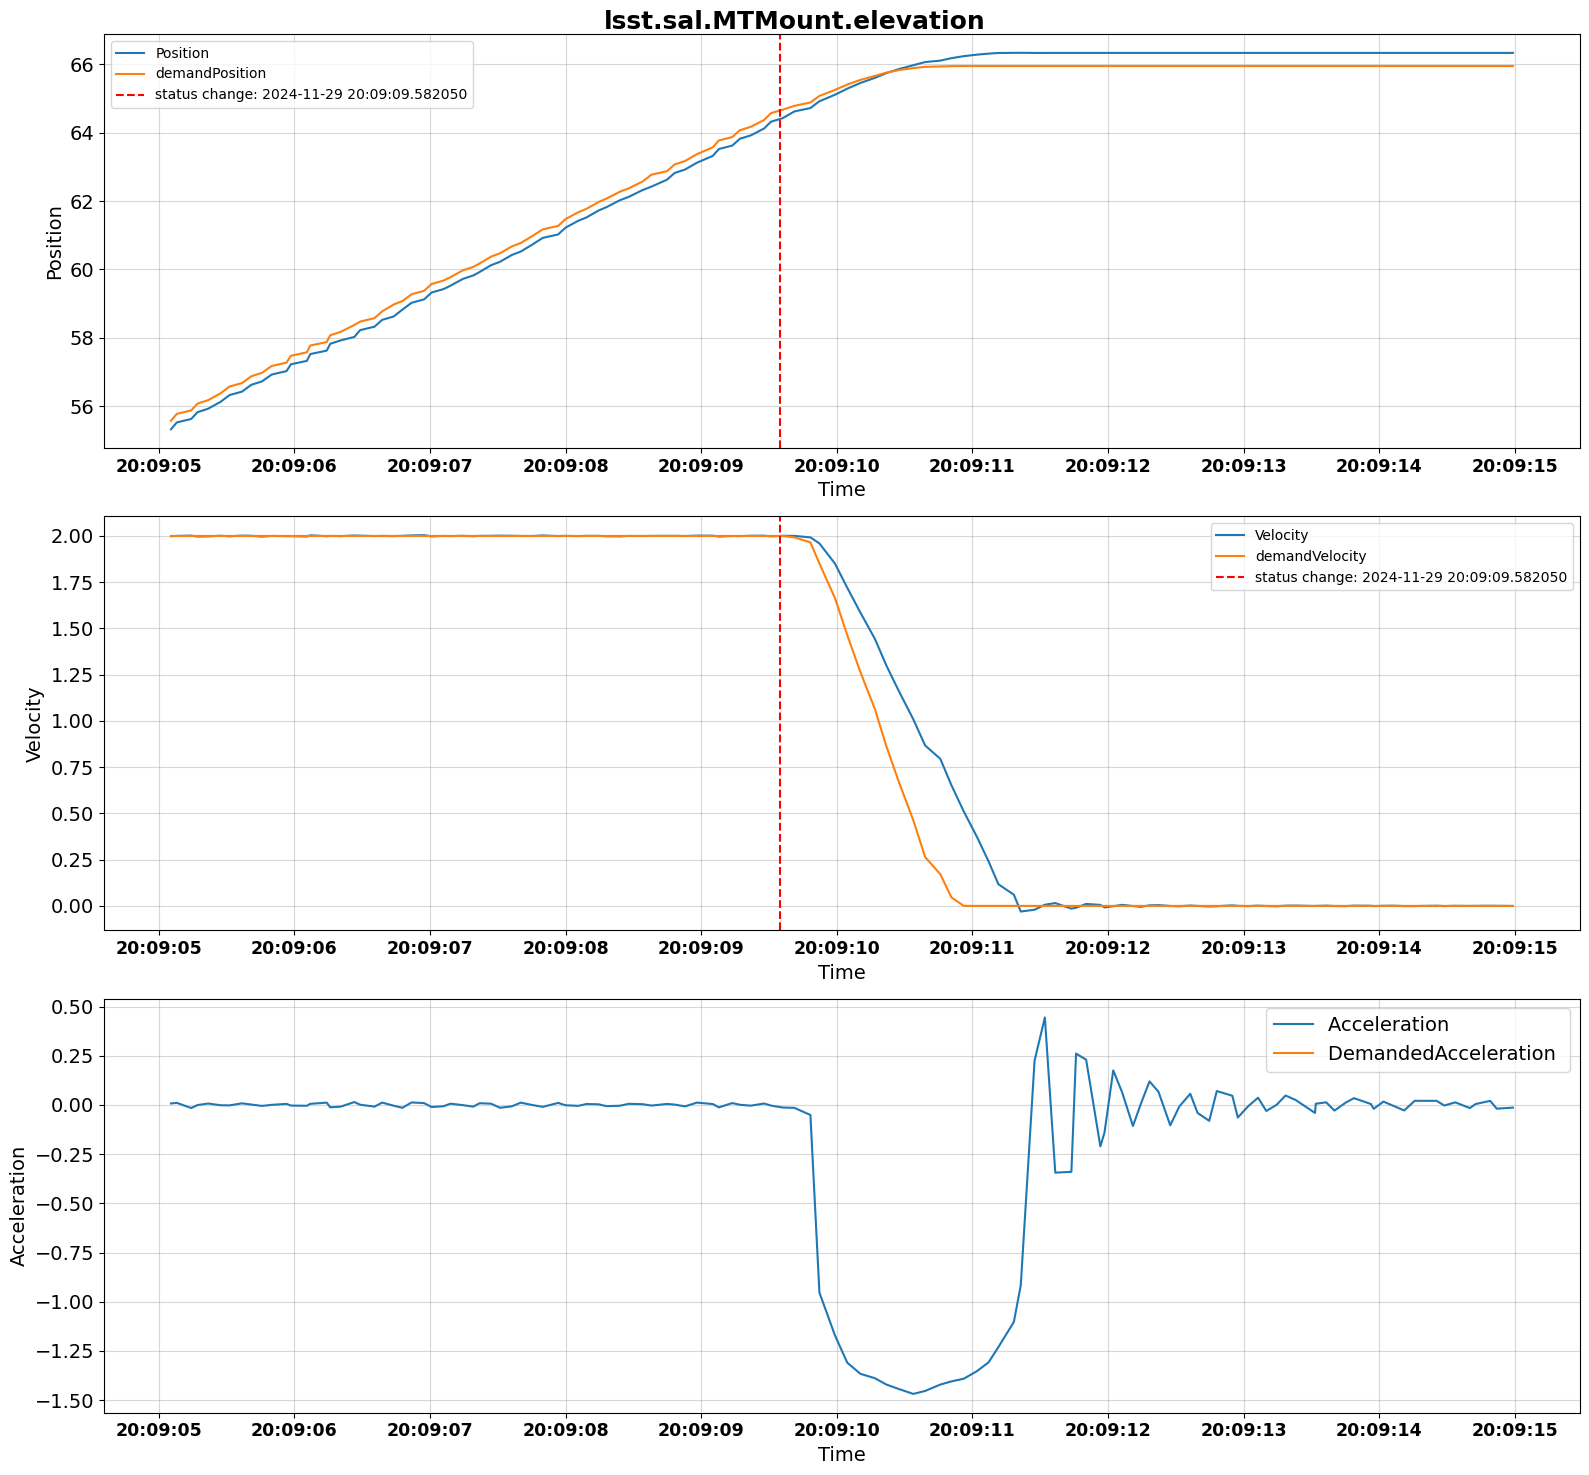
\includegraphics[width=0.45\textwidth]{spa/20_vel_acc_jerk/BLOCK-T240_el_brake_tests.png}
  \caption{TMA Brake Test in Azimuth (left) and Elevation (right).}
  \label{fig:block240_azEl_brake_distance}
\end{figure}

%\subsection{Night Performance}

%Statistical reports/summaries during the night?
%\begin{itemize}
%    \item Measured m1m3 hardpoint histograms min/max HP forces.
%    \item FRACAS-158 / SITCOMTN-081 / SITCOM-1758 - Oscillations on HP forces and on azimuth torques
%\end{itemize}
